%!TEX root = ../template.tex
%%%%%%%%%%%%%%%%%%%%%%%%%%%%%%%%%%%%%%%%%%%%%%%%%%%%%%%%%%%%%%%%%%%
%% chapter1.tex
%% NOVA thesis document file
%%
%% Chapter with introduction
%%%%%%%%%%%%%%%%%%%%%%%%%%%%%%%%%%%%%%%%%%%%%%%%%%%%%%%%%%%%%%%%%%%

\typeout{NT FILE chapter3.tex}%

\chapter{Logic Tools}

In this section...

\section{Iltis Web-Based System for Teaching Logic}
\label{chap:iltis}
Iltis is an interactive online tool designed to help people learning logic from scratch.~\cite{arxivIltisLearning, arxiv} The goal of this tool is to provide a system that supports a wide variety of content (propositional logic, modal logic, and first-order logic) along with a valuable feedback system that helps the learner to better understand their mistakes. This web application is divided into multiple sections. Each section is comprised of a set of tasks (exercises) that increase in difficulty as the learner completes the exercises. For each kind of task, this application provides a custom feedback generator. This feedback can vary depending on the mistakes made by the learner. Some tasks have different levels of feedback that may differ based on the learner’s proficiency. Low feedback levels provide a vaguer hint, and the high ones a more precise and explicit hint. The image below provides a list of the currently available types of exercises in Iltis.

\begin{figure}[htbp]
    \centering
    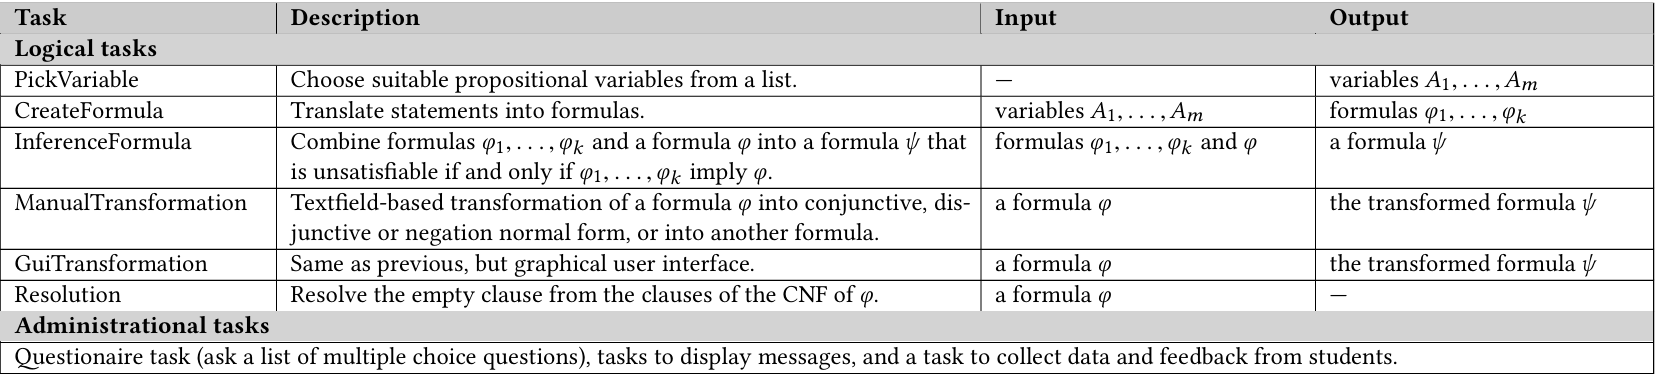
\includegraphics[width=1\linewidth]{Itils_list_of_tasks}
    \caption{List of tasks available in Iltis~\cite{arxiv}.}
\end{figure}

From the teacher’s perspective, this framework provides a way to create more tasks. Teachers can achieve this by using an XML file where they specify a set of tasks, the task type, and a list of feedback generators to be presented to the learner.

\subsection{Feedback}
\label{chap:iltis-feedback}
Iltis allows teachers to associate more than one feedback generator with the task, creating different levels of feedback. Some exercises have feedback generators constructed using reversion rules, providing better and more accurate feedback. In a previous study, researchers collected some of the most frequent mistakes made by learners and built a list of reversion rules. A common example of a reversion rule in the “Propositional Formulas” exercises is to switch the order of the antecedent and consequent in implications. Whenever a learner switches two parameters, the feedback generator tries to apply reversion rules to find the correct solution. If successful, this indicates that the solution is close to the correct one, making it possible to provide more precise feedback based on the applied rule(s). Otherwise, it suggests that the solution is far from the correct one.

\subsection{Conclusion}
There are some positive aspects to consider from this system when developing our own tool, such as the intuitive way (it presents a low learning curve, and it is fundamental for these kinds of tools) that the exercises are presented to the learner, the advanced feedback system, and the easy access to the tool. It also provides a vast set of exercise types and a modular way to create them. On the other hand, teachers need to specify tasks in XML, and this requires some extra knowledge. Some types of exercises are still missing in this tool, like the deduction tree proof. Additionally, this project was developed by a German university and is not open-source, so it cannot be used for further development or expansion.

\section{Logic4Fun}
Logic4Fun is an online tool with a wide range of logical problems and puzzles focused on logical modeling and formalization ~\cite{logic4fun}.
This tool was developed by an Australian university and has been in development since 2001. It was projected to help students practice and develop skills in formalizing logical problems, as this is a challenging topic to teach, and students often struggle with it.

Logic4Fun uses many-sorted first-order logic (MSFO) \footnote{Many-sorted first-order logic is an extension of first-order logic (FOL). In FOL, all variables 
come from the same domain limiting flexibility when modeling exercises with multiple distinct domains. MSFO extends this by allowing the assignment of types (or sorts) to variables and predicates, making the language more expressive.}language to express the problems. It has a solver that takes as input a set of formulas and searches for finite models of this set. This tool presents a web page with different levels of problems: Beginner, Intermediate, Advanced, Expert, and Logician, with increasing complexity. It starts with trivial exercises to help students better understand how to use the site (declare vocabulary, set constraints, and read the solver output) and progresses to more complex and challenging exercises that require a strong background in logic. One of the key advantages of using this tool is the ability to receive immediate and accurate feedback, in contrast with traditional teaching methods. This helps keep students motivated and encourages them to invest more time and effort into solving problems. This site also allows users to enroll in a course by using the credentials provided by the teacher.

\subsection{Feedback}
Logic4Fun tracks two kinds of errors: syntactic and semantic. Syntactic errors are mistakes in the structure or arrangement of words that violate the grammar rules of the language. These errors can be captured by the parser or type checker. When a user attempts to submit an exercise with syntactic errors, a message is presented with some suggestions. When the type checker detects an error, it provides more information, especially about the expected and provided types. Semantic errors are mistakes in logic or meaning in a programming language that occur in program execution. Since there are no predefined solutions, these errors are harder to classify and to deal with. Given these difficulties, Logic4fun simply indicates whether the solution is correct or not. To address the lack of feedback, they created a diagnostic tool to provide more informative responses to the users when a solution cannot be found. There are two approaches to give information provided by the diagnostic tool: using approximate models and using unsatisfiable cores.
\begin{itemize}
    \item In the approximate models approach, the solver starts by marking some unsatisfied constraints as "soft" and then attempts to satisfy as many as possible. Then a user can adjust constraints and rerun the solver, iterating to find the optimal approximations.
    \item In the unsatisfiable cores approach, the solver can try to identify groups of unsatisfied constraints that are causing the problem. Each group must contain at least one contradiction, giving useful clues for troubleshooting the problem. 
\end{itemize}

\subsection{Conclusion}
Logic4Fun has several positive aspects, such as allowing exercises to be saved, enabling users to pause their work and resume it later, progressively increasing the difficulty of exercises, helping users integrate with the tool, and incorporating a diagnostic tool to address the lack of feedback. It has a class system where professors can invite their students to enroll. However, it only provides a restricted range of exercises based on first-order logic. It has some limitations with the solver's performance (the number of models presented to the user is restricted), and it is still facing issues with feedback. Sometimes, the reported errors are overly detailed or unclear, which can become frustrating for the users.

%\section{Iltis}
%\subsection{Conclusion}

\section{Summary}